\newpage
\subsection{Prototype 2}

\subsubsection{Presentation}
\textbf{Tools:} balsamiq

\paragraph{Rationale}
This prototype is a hierarchical design displaying each screen as a series of
steps which the user must progress through before searching. This prototype
also focuses on a very simple, easy to use interface.

Choose all criteria before searching

\paragraph{Home Screen}
\marginpar{%
	\begin{overpic}[width=0.8\marginparwidth]
		{img/firstPrototypes/Pro2Home_Screen}
		% \put(-7,94){\framebox{1}}
		% \put(62,70){\framebox{2}}
		% \put(3,22){\framebox{3}}
		% \put(46,23){\framebox{3}}
		% \put(62,92){\framebox{4}}
		% \put(5,45){\framebox{5}}
	\end{overpic}
	\captionof{figure}{The home screen}\label{fig:Pro2Home_Screen}
}

The home screen offers a choice of three menus

\begin{enumerate}
	\item Make a booking; takes users to the hierarchy of search screens to
		enter their criteria
	\item Change a booking; takes the user to a screen which allows them to
		change their criteria if alternative results permit it
	\item Cancel booking; takes the user to a screen of their current bookings
		and the user can select which booking they would like to cancel.
		Whether a refund is possible would depend on the sport centre
\end{enumerate}

\paragraph{Search screen 1}
% \marginpar{%
% 	\begin{overpic}[width=\marginparwidth]
% 		{img/firstPrototypes/Pro2First_Screen}
% 		% \put(-7,94){\framebox{1}}
% 		% \put(62,70){\framebox{2}}
% 		% \put(3,22){\framebox{3}}
% 		% \put(46,23){\framebox{3}}
% 		% \put(62,92){\framebox{4}}
% 		% \put(5,45){\framebox{5}}
% 	\end{overpic}
% 	\captionof{figure}{First search screen}\label{fig:Pro2First_Screen}
% }

On selecting `Make a booking', the user will be directed to the initial search
screen which will be the first step in their search

\begin{figure}[htpb]
    \centering
    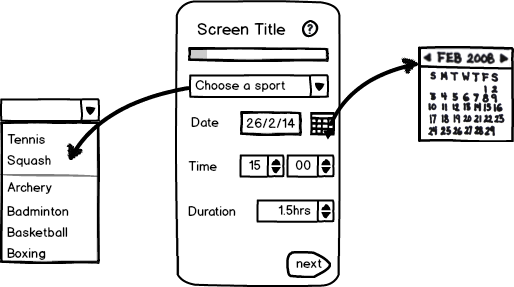
\includegraphics[width=0.8\linewidth]{img/firstPrototypes/Pro2First_Screen}
    \caption{img/firstPrototypes/Pro2FirstScreen
    }\label{fig:img/firstPrototypes/Pro2First_Screen}
\end{figure}

\begin{enumerate}
	\item The help button takes the user to a guide on how to complete the
		current page along with FAQ's.
	\item The progress bar shows the user how far along they are in the search
		process.
	\item The user can choose which sport they would like to play from a drop
		down menu. The drop down menu shows recent search results at the top,
		then list all available sports in alphabetical order.
	\item The user must press on the calendar icon which will present them with
		a calendar to select which date they would like to play.
	\item The time is chosen by selecting the hour and minutes from drop down
		bars.
	\item The user can select how long they would like to play for, chosen from
		a drop down bar with half hour intervals.
	\item Takes the user to the next step in the search process.
\end{enumerate}

\paragraph{Search screen 2}
\marginpar{%
	\begin{overpic}[width=0.8\marginparwidth]
		{img/firstPrototypes/Pro2Second_Screen}
		% \put(-7,94){\framebox{1}}
		% \put(62,70){\framebox{2}}
		% \put(3,22){\framebox{3}}
		% \put(46,23){\framebox{3}}
		% \put(62,92){\framebox{4}}
		% \put(5,45){\framebox{5}}
	\end{overpic}
	\captionof{figure}{Second search screen}\label{fig:Pro2Second_Screen}
}

The next screen focuses on location.

\begin{enumerate}
	\item The search box allows the user to specify their location by either
		town, city or postcode. When the user begins to type a location, the
		system will suggest locations based on what they have already typed
	\item The user can use a horizontal slider to specify how far they are
		willing to travel to play the sport
	\item If the user requires disables access they can tick the checkbox and
		the results will only show sports centres which are wheelchair
		accessible
\end{enumerate}

\paragraph{Search Screen 3}
\marginpar{%
	\begin{overpic}[width=0.8\marginparwidth]
		{img/firstPrototypes/Pro2Third_Screen}
		% \put(-7,94){\framebox{1}}
		% \put(62,70){\framebox{2}}
		% \put(3,22){\framebox{3}}
		% \put(46,23){\framebox{3}}
		% \put(62,92){\framebox{4}}
		% \put(5,45){\framebox{5}}
	\end{overpic}
	\captionof{figure}{Third search screen}\label{fig:Pro2Third_Screen}
}
The user is then brought to the final search screen where they may be able to
get discounts

\begin{enumerate}
	\item Numeric stepper to specify how many people the booking is for.
	\item The user may be eligible for discounts if they are a child, student
		or pensioner. They can tick the suitable checkboxes if they fall into
		any of these categories.
	\item If the user has a strict budget, they can choose to only see results
		which do not exceed a  particular price.
	\item Pressing the search button takes the user to a screen displaying the
		results of the search.
\end{enumerate}

\paragraph{Results Screen}
\marginpar{%
	\begin{overpic}[width=\marginparwidth]
		{img/firstPrototypes/Pro2Results_screen}
		% \put(-7,94){\framebox{1}}
		% \put(62,70){\framebox{2}}
		% \put(3,22){\framebox{3}}
		% \put(46,23){\framebox{3}}
		% \put(62,92){\framebox{4}}
		% \put(5,45){\framebox{5}}
	\end{overpic}
	\captionof{figure}{Results screen}\label{fig:Pro2Results_Screen}
}
Screen showing the results of the search

\begin{enumerate}
	\item The user can sort the results by distance, price or time.
	\item If the results are not suitable, the user may wish to change their
		search criteria, the `amend search' button will take them back to the
		first search screen where they can alter their original preferences.
	\item Each result informs the user of the time, date, venue name, distance
		from the venue and the price. The price shows the total price for all
		people. The user can scroll down the page to view all matching results.
	\item Pressing the buttons displaying the price will take the user to a
		more detailed description of the booking and a link to an external pay
		site or the website of that sports facility to pay for the booking.
\end{enumerate}

\newpage
\subsubsection{Evaluation}

\begin{center}
	\begin{adjustwidth*}{}{-3cm}
	\renewcommand{\arraystretch}{2}
	\begin{longtable}{@{\extracolsep{\fill}}p{0.3\linewidth} c p{0.6\linewidth}}
		\toprule
		\textbf{Criteria} & \textbf{Rating} & \textbf{Comment}\\
		\midrule
		Visibility of system status & $+$ & Each screen shows the user their
		progress in the search process \\

		Match between system and the real world & $+$ & Each field is self
		explanatory and is clear what is asked of the user.  \\

		User control and freedom & $-$ & The hierarchical nature of the system
		prevents the user from switching screens easily. If they choose to go
		back they will lose the information they have already typed on the
		screen they left. Freedom is also restricted as the user is required to
		fill all fields. For example they must pick a particular sport at a
		particular time. \\

		Consistency and standards & $-$ & The way users specify their criteria
		varies throughout the search, for example horizontal sliders and
		steppers to achieve numerical values. Although this would not reduce
		the clarity of what is asked of the user. \\

		Error prevention & + & Due to the large buttons and very simple
		interface, there is very little chance of user error. Although the drop
		down menus could get a little fiddly. If the user does accidentally
		book the wrong option, they may have the opportunity to change or
		cancel this booking. \\

		Recognition rather than re-call & $+$ & Information required on the
		current search screen does not depend on information on the previous
		screen. \\

		Flexibility and efficiency use & 0 & Lacks efficiency due to the fact
		that the user must progress through all search screens filling in all
		fields before they can search. \\

		Aesthetic and minimalist design & $+$ & The design is very simple so as
		not to cause any confusion to the user \\

		Help users recognize, diag-nose, and recover from errors & $+$\ & If
		the user tries to move to the next screen having not filled a field or
		filled it incorrectly,  they will be shown a descriptive error message
		in red above that field \\

		Help and documentation & $+$ & The help button displayed on every
		screen takes the user to a guide on how to complete the current page
		along with FAQ's \\
		\bottomrule
	\end{longtable}
\end{adjustwidth*}
\end{center}

\begin{center}
	\begin{adjustwidth*}{}{-3cm}
	\renewcommand{\arraystretch}{2}
	\begin{longtable}{@{\extracolsep{\fill}}p{0.3\linewidth} c p{0.6\linewidth}}
		\toprule
		\textbf{Scenario} & \textbf{Rating} & \textbf{Comment}\\
		\midrule
		\midrule
		\multicolumn{3}{l}{\textbf{Elderly}}\\
		\cmidrule(r){1-3}
		Searching for new sports in the area and notifying his wife of the
		booking. & $-$ & Howard may find using the drop down menus difficult
		with his osteoarthritis. There is no feature to notify people of the
		booking \\

		Racquet sport with 4 friends on Friday & 0 & Can select four people
		to play using drop down menu. Would have to specify which racquet sport
		he wishes to play. No bulk book feature. \\

		Swimming nearby with knee pain & $+$ & If Howard does not wish to
		travel far he can either filter the results by distance or specify a
		maximum distance he is willing to travel (search screen2). If Howards
		knee pain is particularly bad he may wish to swim somewhere which
		doesn't require climbing any stairs. He can do this by ticking the
		wheelchair accessible checkbox. \\

		\midrule
		\multicolumn{3}{l}{\textbf{Working}}\\
		\cmidrule(r){1-3}
		Team sport on Friday including screen sharing with friends & $-$ & The
		app would not support this scenario as there is no option to search for
		just team sports. There is also no current feature to support screen
		sharing but this could be incorporated into the final design. \\

		Change/cancel booking at late notice & 0 & Janet has this option on
		the home screen. Although the app cannot guarantee the venue allows
		cancellations \\

		Outdoor sport early on Saturday & 0 & Useful as Janet can specify a
		time. But again, there is no flexibility in choosing a sport. \\

		\midrule
		\multicolumn{3}{l}{\textbf{Student}}\\
		\cmidrule(r){1-3}
		Tennis court at specific time & $+$ & This scenario is tailored this
		prototypes design. Jenny can specify that she would like to play tennis
		at a particular time on a particular day and how long she would like to
		play for \\

		Weekday evening session must be on clay & 0 & This could be something
		to incorporate on the screen showing the booking in more detail, along
		with other information such as court number \\

		Weekly practice with friend with reminders & $-$ & There is no
		notification feature with this prototype. The regular weekly booking
		feature could also be something that is incorporated in the screen
		showing more detail about the booking. \\

		\midrule
		\multicolumn{3}{l}{\textbf{Student}}\\
		\cmidrule(r){1-3}
		Outdoor sport close to home or on a bus route with coach & $-$ & No
		feature showing any transport routes. Joe would also have to specify
		which outdoor sport he is interested in playing \\

		Booking several squash courts for after school tournament & $-$ &
		With the current design, Joe would have to use the number of players
		field (4 people = 1 court) to portray how many courts he needs. He can
		specify how long they need the courts based on how long they think
		tournament will last. However he would need to choose a particular day.
		\\

		Looking for high quality tennis court & $-$ & There is currently no
		way of finding the quality of the sport facilities. Pete can however,
		use the sliders to increase the maximum distance and price they are
		willing to pay. \\
		\bottomrule
	\end{longtable}
	\end{adjustwidth*}
\end{center}
